% Conceptual process flow at the brief's 5,000 t/month of Tiros run-of-mine ore.
% Stream values: model v0.7 (Model tab, Case 1), monthly = yearly / 12. Splits from the BK19 bench test (Needs testing).
\documentclass[tikz,border=4pt]{standalone}
\usepackage[T1]{fontenc}
\usepackage[scaled=0.92]{helvet}
\renewcommand\familydefault{\sfdefault}
\usepackage[version=4]{mhchem}
\usetikzlibrary{positioning,arrows.meta,calc,fit,backgrounds}
% Team palette (docs/style-guide.md)
\definecolor{ink}{HTML}{26313A}
\definecolor{oxide}{HTML}{1E5245}
\definecolor{sand}{HTML}{F6EFDF}
\definecolor{band}{HTML}{F3F5F2}
\definecolor{muted}{HTML}{6B7780}
\definecolor{rule}{HTML}{C9CFC9}
\definecolor{amber}{HTML}{9A6A14}
\definecolor{brick}{HTML}{A33B2B}

\begin{document}
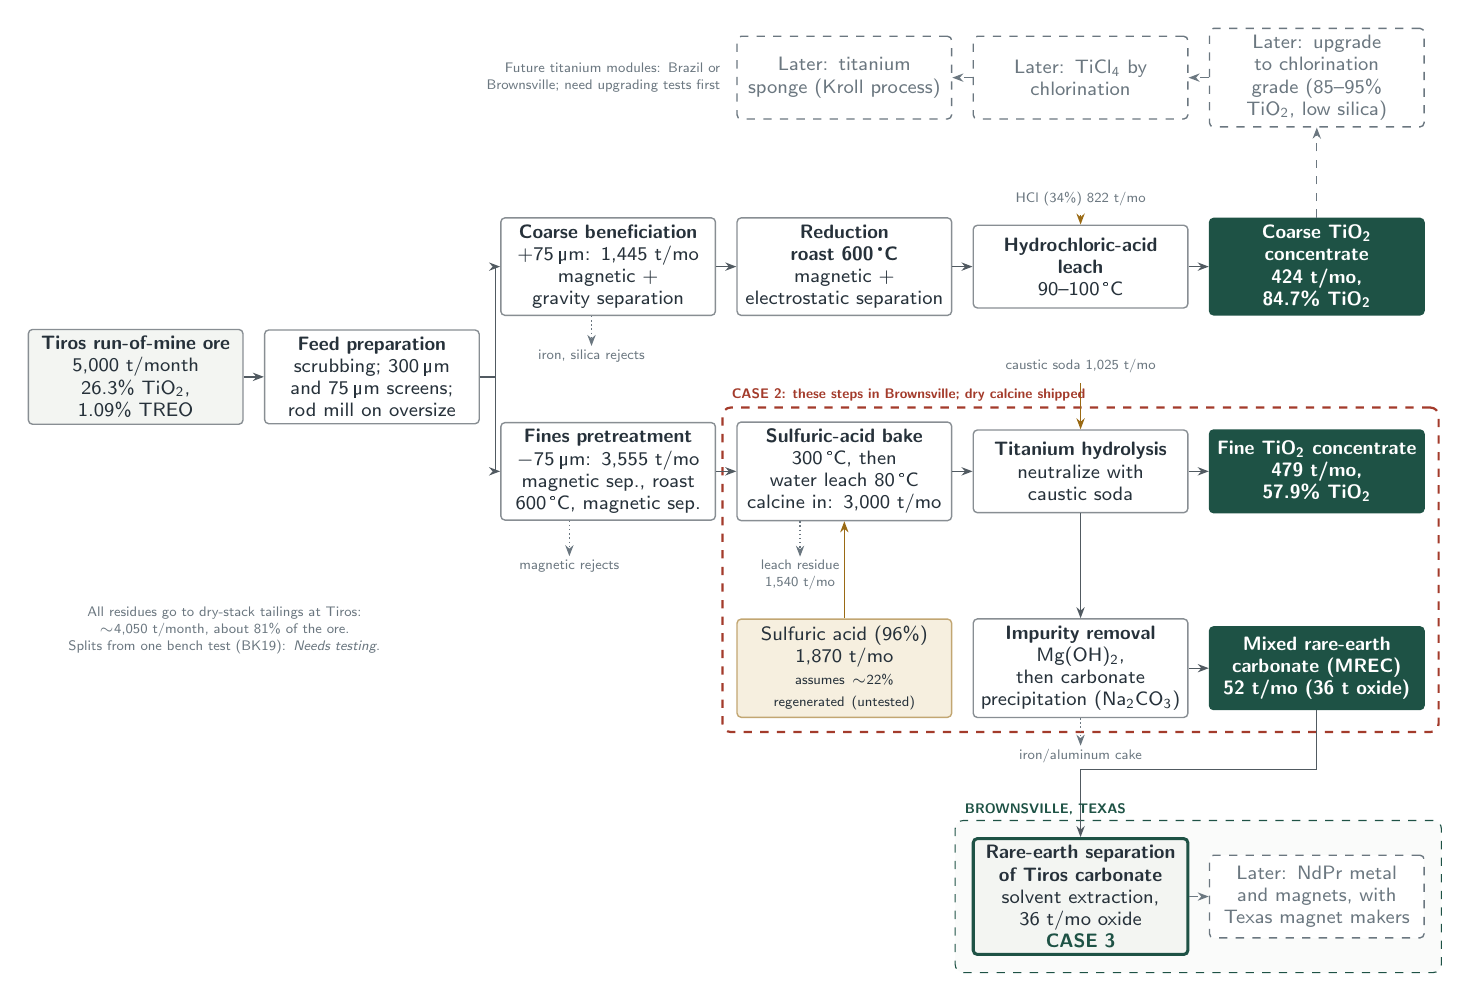
\begin{tikzpicture}[
  font=\scriptsize\sffamily, >={Stealth[length=4pt]}, line width=0.5pt, color=ink,
  box/.style={rectangle, rounded corners=1.5pt, draw=ink!55, fill=white, text width=2.55cm, align=center,
              minimum height=1.05cm, inner sep=2.5pt, execute at begin node={\hyphenpenalty=10000\exhyphenpenalty=10000}},
  prod/.style={box, fill=oxide, draw=oxide, text=white, font=\scriptsize\sffamily\bfseries},
  reag/.style={box, fill=sand, draw=amber!60, minimum height=0.8cm},
  future/.style={box, dashed, draw=muted, text=muted},
  module/.style={box, draw=oxide, line width=1.1pt, fill=band},
  flow/.style={->, draw=ink!80},
  stub/.style={->, draw=muted, densely dotted},
  note/.style={font=\tiny\sffamily, text=muted, align=center}
]
% ---------------- Brazil: feed preparation
\node[box, fill=band] (rom) at (0,1.2) {\textbf{Tiros run-of-mine ore}\\5,000 t/month\\26.3\% \ce{TiO2}, 1.09\% TREO};
\node[box] (prep) at (3,1.2) {\textbf{Feed preparation}\\scrubbing; 300\,\textmu m and 75\,\textmu m screens; rod mill on oversize};
% ---------------- coarse circuit
\node[box] (c1) at (6,2.6) {\textbf{Coarse beneficiation}\\+75\,\textmu m: 1,445 t/mo\\magnetic + gravity separation};
\node[box] (c2) at (9,2.6) {\textbf{Reduction roast 600\,\textdegree C}\\magnetic + electrostatic separation};
\node[box] (c3) at (12,2.6) {\textbf{Hydrochloric-acid leach}\\90--100\,\textdegree C};
\node[prod] (pc) at (15,2.6) {Coarse \ce{TiO2} concentrate\\424 t/mo, 84.7\% \ce{TiO2}};
% ---------------- fines circuit
\node[box] (f1) at (6,0) {\textbf{Fines pretreatment}\\$-$75\,\textmu m: 3,555 t/mo\\magnetic sep., roast 600\,\textdegree C, magnetic sep.};
\node[box] (f2) at (9,0) {\textbf{Sulfuric-acid bake}\\300\,\textdegree C, then water leach 80\,\textdegree C\\calcine in: 3,000 t/mo};
\node[box] (f3) at (12,0) {\textbf{Titanium hydrolysis}\\neutralize with caustic soda};
\node[prod] (pf) at (15,0) {Fine \ce{TiO2} concentrate\\479 t/mo, 57.9\% \ce{TiO2}};
\node[box] (l1) at (12,-2.5) {\textbf{Impurity removal}\\\ce{Mg(OH)2}, then carbonate precipitation (\ce{Na2CO3})};
\node[prod] (pm) at (15,-2.5) {Mixed rare-earth carbonate (MREC)\\52 t/mo (36 t oxide)};
% ---------------- reagents
\node[reag] (acid) at (9,-2.5) {Sulfuric acid (96\%)\\1,870 t/mo\\{\tiny assumes $\sim$22\% regenerated (untested)}};
\node[note, anchor=south] (naoh) at (12,1.12) {caustic soda 1,025 t/mo};
\node[note, anchor=south] (hcl) at (12,3.25) {HCl (34\%) 822 t/mo};
% ---------------- flows
\draw[flow] (rom) -- (prep);
\draw[flow] (prep.east) -- ++(0.2,0) |- (c1.west);
\draw[flow] (prep.east) -- ++(0.2,0) |- (f1.west);
\draw[flow] (c1) -- (c2); \draw[flow] (c2) -- (c3); \draw[flow] (c3) -- (pc);
\draw[flow] (f1) -- (f2); \draw[flow] (f2) -- (f3); \draw[flow] (f3) -- (pf);
\draw[flow] (f3) -- (l1); \draw[flow] (l1) -- (pm);
\draw[flow, draw=amber] (acid) -- (f2);
\draw[flow, draw=amber] (naoh.south) -- (f3.north);
\draw[flow, draw=amber] (hcl.south) -- (c3.north);
% ---------------- residue stubs
\draw[stub] ([xshift=-6pt]c1.south) -- ++(0,-0.38) node[below, note, inner sep=1pt]{iron, silica rejects};
\draw[stub] ([xshift=-14pt]f1.south) -- ++(0,-0.45) node[below, note, inner sep=1pt]{magnetic rejects};
\draw[stub] ([xshift=-16pt]f2.south) -- ++(0,-0.45) node[below, note, inner sep=1pt, text width=1.3cm]{leach residue 1,540 t/mo};
\draw[stub] (l1.south) -- ++(0,-0.35) node[below, note, inner sep=1pt]{iron/aluminum cake};
\node[note, text width=4.6cm, anchor=north west] at (-1.3,-1.6) {All residues go to dry-stack tailings at Tiros:\\$\sim$4,050 t/month, about 81\% of the ore.\\Splits from one bench test (BK19): \textit{Needs testing}.};
% ---------------- Case 2 boundary
\begin{scope}[on background layer]
\node[draw=brick, dashed, line width=0.8pt, rounded corners=3pt, inner sep=5pt,
      fit=(f2)(f3)(pf)(l1)(pm)(acid)] (case2) {};
\end{scope}
\node[anchor=south west, font=\tiny\sffamily\bfseries, text=brick, inner sep=1.5pt]
     at ([xshift=2pt]case2.north west) {CASE 2: these steps in Brownsville; dry calcine shipped};
% ---------------- Brownsville modules (Case 3 and later)
\node[module] (sep) at (12,-5.4) {\textbf{Rare-earth separation of Tiros carbonate}\\solvent extraction, 36 t/mo oxide\\{\color{oxide}\textbf{CASE 3}}};
\node[future] (mag) at (15,-5.4) {Later: NdPr metal and magnets, with Texas magnet makers};
\draw[flow] (pm.south) -- ++(0,-0.75) -| (sep.north);
\draw[flow, dashed, draw=muted] (sep) -- (mag);
\begin{scope}[on background layer]
\node[draw=oxide, dashed, rounded corners=3pt, inner sep=6pt, fit=(sep)(mag), fill=band!40] (bv) {};
\end{scope}
\node[anchor=south west, font=\tiny\sffamily\bfseries, text=oxide, inner sep=1.5pt]
     at ([xshift=2pt]bv.north west) {BROWNSVILLE, TEXAS};
% ---------------- future titanium modules
\node[future] (up) at (15,5.0) {Later: upgrade to chlorination grade (85--95\% \ce{TiO2}, low silica)};
\node[future] (ticl) at (12,5.0) {Later: \ce{TiCl4} by chlorination};
\node[future] (sponge) at (9,5.0) {Later: titanium sponge (Kroll process)};
\draw[flow, dashed, draw=muted] (pc) -- (up);
\draw[flow, dashed, draw=muted] (up) -- (ticl);
\draw[flow, dashed, draw=muted] (ticl) -- (sponge);
\node[note, anchor=east, text width=3.4cm, align=right] at (7.55,5.0) {Future titanium modules: Brazil or Brownsville; need upgrading tests first};
\end{tikzpicture}
\end{document}
